\documentclass[a4paper]{book}
\usepackage[a4paper]{geometry}
\usepackage[czech]{babel}
\usepackage[IL2]{fontenc}
\usepackage[utf8]{inputenc}
\usepackage{pstricks}
\usepackage{amsmath, amssymb}
\usepackage{graphicx}
\usepackage{pdfpages}
\usepackage{mathrsfs}

\usepackage{fancyhdr}
\pagestyle{fancy}
\fancyhead{}
\fancyhead[LE,RO]{\thepage}
\fancyhead[RE]{\leftmark}
\fancyhead[LO]{\rightmark}

%\includeonly{wool_chap1}

\setlength{\unitlength}{1.0mm}
\sloppy

\begin{document}

\newtheorem{definition}{Definice}[chapter]
\newtheorem{theorem}{Věta}[chapter]
\newtheorem{proof}{Důkaz}[chapter]
\newtheorem{example}{Příklad}[chapter]
\newtheorem{corollary}{Tvrzení}[chapter]
\newtheorem{assumption}{Předpoklad}[chapter]

\hyphenation{prav-dě-po-dob-nost prav-dě-po-dob-nost-ní} 

\title{Aplikovaná logistická regrese\\druhé vydání}
\author{David W. Hosmer, Stanley Lemeshow}
\maketitle

\tableofcontents

\chapter{Úvod do logistického regresního modelu}

\section{Úvod}

V případě jednorozměrného lineárního regresního modelu předpokládáme, že střední hodnotu závislé veličiny $Y$ podmíněnou hodnotou $x$ lze vyjádřit jako
\begin{equation}
E(Y | x) = \beta_0 + \beta_1 x,
\end{equation}
kde $E(Y | x)$ může nabývat libovolné hodnoty z intervalu $(-\infty, \infty)$.

V případě logistického regresního modelu má závislá veličina binární charakter, tj. může nabývat pouze dvou hodnot. Její střední hodnota tak omezena na interval $[0, 1]$. To je také patrné z obrázku 1.1, který ilustruje závislost mezi věkem pacienta a ischemickou chorobou srdeční. Z grafu, který má tvar písmene S, je patrné, že se střední hodnota vypočtena pro jednotlivé věkové kohorty postupně blíží jedné. Graf tak můžeme chápat ve smyslu kumulativní pravděpodobnostní funkce náhodné veličiny.

\begin{figure}[htp]
\centering
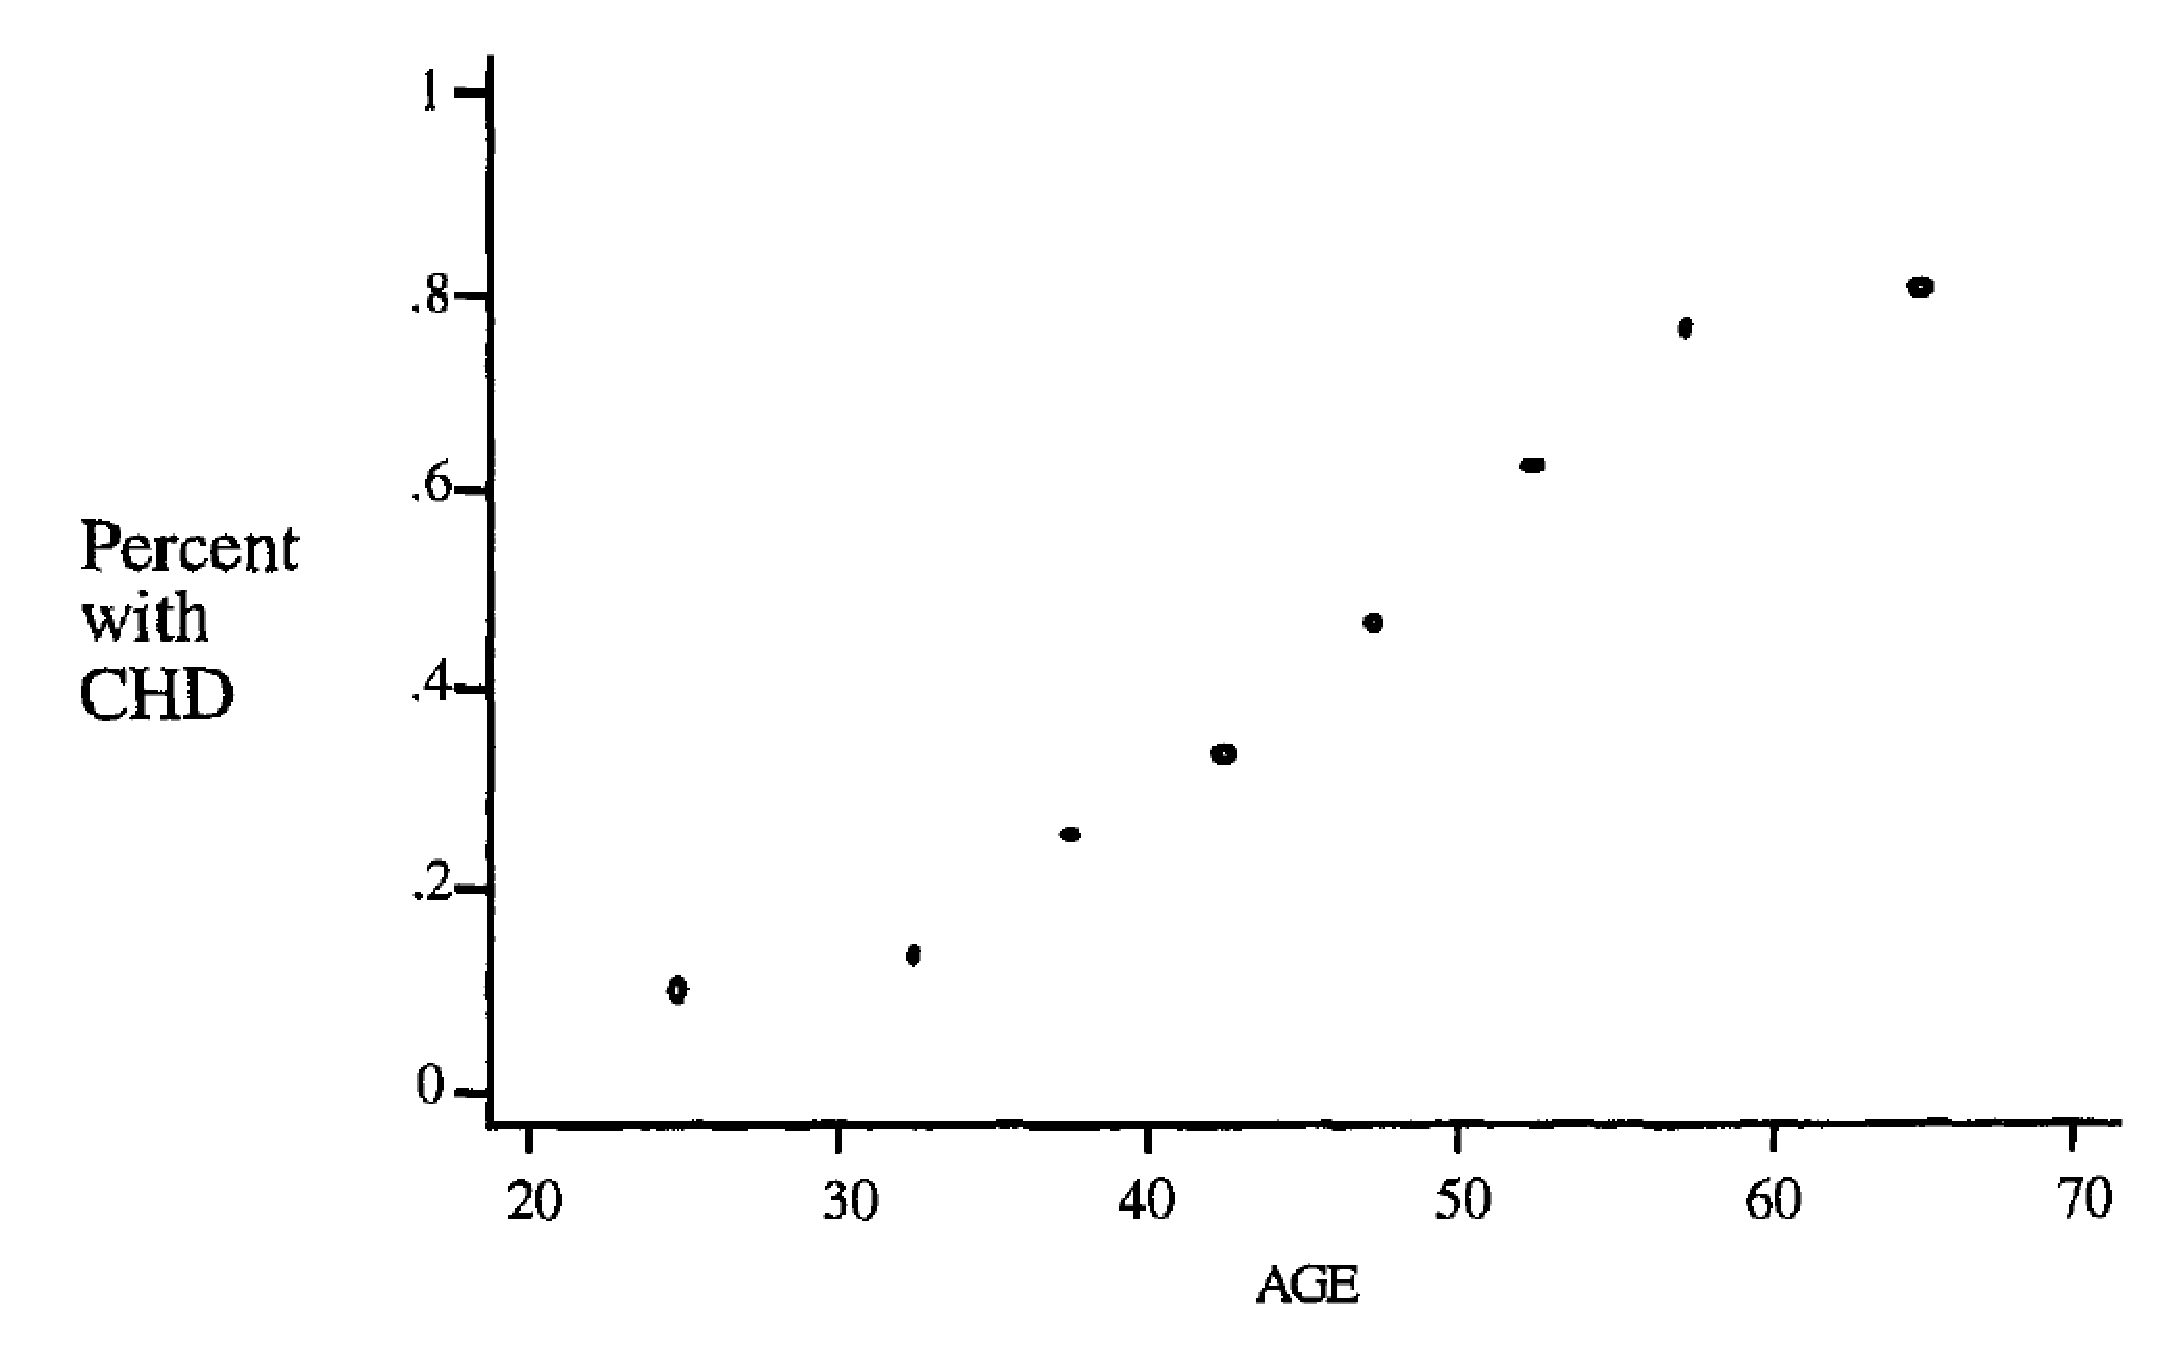
\includegraphics[scale = 0.35]{pictures/fig_1_2.eps}
\caption{Vztah mezi výskytem ischemické poruchy srdeční a věkem pacienta}
\label{fig_1_2}
\end{figure}

V následujícím textu budeme výraz $\pi(x) = E(Y | x)$ používat pro označení střední hodnoty závislé veličiny $Y$ podmíněné hodnotu $x$ pro jednorozměrný logistický regresní model, kde
\begin{equation}
\pi(x) = \frac{e^{\beta_0 + \beta_1 x}}{1 + e^{\beta_0 + \beta_1 x}}.
\end{equation}
Tuto transformaci, která je klíčová pro studium logistického regresního modelu, nazýváme logit transformací a lze ji snadno upravit do tvaru
\begin{equation}
g(x) = \ln \Big[\frac{\pi(x)}{1 - \pi(x)} \Big] = \beta_0 + \beta_1 x.
\end{equation}
Funkce $g(x)$, kterou nazýváme logit funkcí, může nabývat hodnot z intervalu $(-\infty, \infty)$.

Hodnotu závislé veličiny $y$ pro danou hodnotu $x$ můžeme vyjádřit jako $y = \pi(x) + \varepsilon$, kde $\varepsilon$ nabývá dvou stavů. Pokud $y = 1$, pak $\varepsilon = 1 -\pi(x)$ s pravděpodobností $\pi(x)$; pokud $y = 0$, pak $\varepsilon = -\pi(x)$ s pravděpodobností $1 - \pi(x)$.\footnote{Pokud $Y$ nabývá hodnot 0 popř. 1, lze $\pi(x) = E(Y | x)$ interpretovat ve smyslu pravděpodobnosti, s jakou $Y$ nabývá pro dané $x$ hodnoty 1. Pravděpodobnost, s jakou $Y$ nabývá pro dané $x$ hodnoty 0, je pak $1 - \pi(x)$.} Chyba $\varepsilon$ tak sleduje binomické rozdělení s nulovou střední hodnotou a rozptylem $\pi(x)[1 - \pi(x)]$. To je další ze zásadních rozdílů oproti lineárnímu regresnímu modelu, ve kterém chyba $\varepsilon$ sleduje normální rozdělení.

\section{Kalibrace logistického regresního modelu}

Základní metodou odhadu parametrů lineárního regresního modelu je metoda nejmenších čtverců. Podstatou této metody je volba takových hodnot parametrů $\beta_0$ a $\beta_1$, které minimalizují součet kvadrátu odchylek pozorovaných a predikovaných hodnot závislé veličiny $Y$. Tuto metodu však není v případě logistického regresního modelu možné použít.

Obecnější metodou odhadu parametrů je tzv. metoda maximální věrohodnosti, která odhadne hodnoty parametrů tak, aby výsledný model s maximální možnou pravděpodobností replikoval pozorovaná data. Za tímto účelem je třeba definovat tzv. funkci maximální věrohodnosti, která vyjadřuje pravděpodobnost výskytu pozorovaných dat v kontextu uvažovaného modelu jako funkci jeho parametrů.

Uvažujme jednorozměrný logistický regresní model a obecný pár $(x_i, y_i)$. Pokud $y_i = 1$, je kontribuce páru $(x_i, y_i)$ do funkce maximální věrohodnosti rovna $\pi(x)$. Pokud $y_i = 0$, je kontribuce páru $(x_i, y_i)$ do funkce maximální věrohodnosti rovna $1 - \pi(x)$. Tyto dva stavy lze zkombinovat do podoby
\begin{equation}
\pi(x_i)^{y_i}[1 - \pi(x_i)]^{1 - y_i}.
\end{equation}
Pokud předpokládáme, že jednotlivá pozorování představovaná páry $(x_i, y_i)$ jsou vzájemně nezávislá, lze funkci maximální věrohodnosti vyjádřit jako
\begin{equation}
l(\pmb{\beta}) = \prod_{i = 1}^n \pi(x_i)^{y_i}[1 - \pi(x_i)^{1 - y_i}].
\end{equation}
Z matematického a numerického hlediska je však snadnější pracovat s logaritmem funkce maximální věrohodnosti
\begin{equation}
L(\pmb{\beta}) = \ln[l(\pmb{\beta})] = \sum_{i = 1}^n \Big(y_i \ln[\pi(x_i) + (1 - y_i) \ln[1 - \pi(x_i)] \Big),
\end{equation}
kde $\pi(x_i) = \frac{e^{\beta_0 + \beta_1 x_i}}{1 + e^{\beta_0 + \beta_1 x_i}}$. Abychom nalezli hodnotu $\pmb{\beta}$, která maximalizuje $L(\pmb{\beta})$, je třeba nejprve derivovat $L(\pmb{\beta})$ dle $\beta_0$ a $\beta_1$ a tyto derivace položit rovny nule. Výsledné rovnice, které nazýváme rovnicemi maximální věrohodnosti, mají podobu
\begin{equation}
\sum_{i = 1}^n [y_i - \pi(x_i)] = 0
\end{equation}
a
\begin{equation}
\sum_{i = 1}^n x_i [y_i - \pi(x_i)] = 0.
\end{equation}
Rovnice maximální věrohodnosti jsou nelineární v parametrech $\beta_0$ a $\beta_1$, a proto je třeba je řešit iteračně pomocí optimalizační metody. Hodnotu $\pmb{\beta}$, která je řešením výše uvedených rovnic, značíme $\hat{\pmb{\beta}}$ a nazýváme ji odhadem maximální věrohodnosti. Podobně je $\hat{\pi}(x_i)$ odhadem maximální věrohodnosti pro $\pi(x_i)$, a platí
\begin{equation}
\hat{\pi}(x_i) = \frac{e^{\hat{\beta}_0 + \hat{\beta}_1 x_i}}{1 + e^{\hat{\beta}_0 + \hat{\beta}_1 x_i}}.
\end{equation}
Odhadnutá logit funkce pak má tvar
\begin{equation}
\hat{g}(x_i) = \hat{\beta}_0 + \hat{\beta}_1 x_i.
\end{equation}

Rovnici (1.7) lze také vyjádřit ve tvaru
\begin{equation}
\sum_{i = 1}^n y_i = \sum_{i = 1}^n \hat{\pi}(x_i),
\end{equation}
což lze interpretovat tak, že součet pozorovaných hodnot veličiny $y$ je roven součtu predikovaných hodnot.

\section{Testy významnosti odhadnutých parametrů}

\subsection{Věrohodnostní poměrový test}

Při posuzování statistické významnosti odhadnutého parametru porovnáváme pozorované hodnoty s predikovanými hodnotami získaných na základě dvou logistických regresních modelů, z nichž jeden zahrnuje zkoumanou veličinu a druhý nikoliv. Samotné porovnání modelů je pak založené na porovnání logaritmů jejich funkce maximální věrohodnosti. Pro lepší pochopení principu je užitečné o pozorovaných hodnotách přemýšlet jako o hodnotách predikovaných tzv. saturovaným model. Saturovaný logistický regresní model je takový model, který obsahuje tolik parametrů kolik je pozorovaných párů $(x_i, y_i)$.\footnote{Jednoduchým příkladem saturovaného modelu je kalibrace jednorozměrného lineárního regresního modelu na dvou pozorováních.} Porovnání pozorovaných a predikovaných hodnot je pak založeno na statistice
\begin{equation}
D = -2 \ln \Big[\frac{\textit{hodnota funkce maximální věrohodnosti kalibrovaného modelu}}{\textit{hodnota funkce maximální věrohodnosti saturovaného modelu}}\Big],
\end{equation}
kterou nazýváme věrohodnostním poměrem (likelihood ratio) a test na ní založený pak věrohodnostním poměrovým testem (likelihood ratio test). S využitím (1.6), (1.12) a skutečnosti, že pro hodnotu věrohodnostní funkce saturovaného modelu platí
\begin{equation}
l(\textit{saturovaný model}) = \prod_{i = 1}^n y_i^{y_i}(1 - y_i)^{1 - y_i},
\end{equation}
lze statistiku $D$ vyjádřit jako
\begin{equation}
D = -2 \sum_{i = 1}^n \Big[u_i \ln\Big( \frac{\hat{\pi}_i}{y_i} \Big) + (1 - y_i) \ln \Big( \frac{1 - \hat{\pi}_i}{1 - y_i} \Big) \Big],
\end{equation}
kde $\hat{\pi}_i = \hat{\pi}(x_i)$. Pokud si dále uvědomíme, že hodnota věrohodnostní funkce saturovaného modelu je vždy rovna jedné\footnote{Toto tvrzení lze snadno ověřit dosazením $y_i = 1$ a $y_i = 0$ do (1.13).}, lze (1.12) zjednodušit do podoby
\begin{equation}
D = -2 \ln (\textit{hodnota funkce maximální věrohodnosti kalibrovaného modelu}).
\end{equation}

Pro účely zhodnocení významnosti nezávislé veličiny pak porovnáváme věrohodnostní poměr $D$ pro model s a bez uvažované veličiny, tj.
\begin{multline}
G = D(\textit{hodnota funkce maximální věrohodnosti bez uvažované veličiny}) - \\
D(\textit{hodnota funkce maximální věrohodnosti s uvažovanou veličinou}),
\end{multline}
což lze dále upravit na
\begin{equation}
G = -2 \ln \left[\frac{\textit{hodnota funkce maximální věrohodnosti bez uvažované veličiny}}{\textit{hodnota funkce maximální věrohodnosti s uvažovanou veličinou}}\right].
\end{equation}
Lze snadno dokázat, že v případě modelu, který zahrnuje pouze parametr $\beta_0$, je odhad tohoto parametru roven $\ln(n_1 / n_0)$, kde $n_1 = \sum_{i = 1}^n y_i$ a $n_0 = \sum_{i = 1}^n (1 - y_i)$ a predikovaná hodnota má charakter konstanty $n_1 / n$. V tomto případě pak pro námi uvažovaný jednorozměrný logistický regresní model platí
\begin{equation}
G = -2 \ln \left[\frac{\Big(\frac{n_1}{n}\Big)^{n_1}\Big(\frac{n_0}{n}\Big)^{n_0}}{\prod_{i = 1}^n \hat{\pi}_i (1 - \hat{\pi}_i)^{1 - y_i}}\right].
\end{equation}

Při platné nulové hypotéze $H_0: \beta_1 = 0$ sleduje $G$ chi-kvadrát rozdělení s jedním stupněm volnosti.

\subsection{Waldův test}

Alternativou k věrohodnostnímu poměrovému testu je Waldův test, který poměřuje hodnotu odhadnutého parametru $\hat{\beta}_1$ k jeho směrodatné odchylce. Výsledný poměr
\begin{equation}
W = \frac{\hat{\beta}_1}{\widehat{se}(\hat{\beta}_1)}
\end{equation}
při platnosti nulové hypotézy $H_0: \beta_1 = 0$ sleduje standardní normální rozdělení. Nevýhodou Waldova testu bohužel je, že často nezamítne nulovou hypotézu ani v případě, kdy je odhadnutý parametr významný. Proto je vhodnější používat věrohodnostní poměrový test.

\subsection{Skóre test}

Dalším možným testem významnosti parametru je tzv. skóre test, jehož hlavní výhodou je nižší výpočetní náročnost. Test je založen na teorii pravděpodobnostního rozdělení derivace logaritmu věrohodnostní funkce. Konkrétně v případě jednorozměrného logistického regresního modelu je test založen na znalosti pravděpodobnostního rozdělení derivace (1.8) podmíněné derivací (1.7). Test používá hodnotu rovnice (1.8) vypočtenou s pomocí $\beta_0 = \ln(n_1 / n_0)$ a $\beta_1 = 0$. Jak již bylo zmíněno dříve, platí pro tento případ $\hat{\pi} = n_1 / n = \overline{y}$. Dále lze dokázat, že odhadovaný rozptyl je $\overline{y}(1 - \overline{y}) \sum (x_i - \overline{x})^2$. To vede ke statistice
\begin{equation}
ST = \frac{\sum_{i = 1}^n x_i (y_i - \overline{y})}{\sqrt{\overline{y}(1 - \overline{y}) \sum_{i = 1}^n (x_i - \overline{x})^2}},
\end{equation}
která opět sleduje standardizované normální rozdělení. Opět nicméně platí, že věrohodnostní poměrový test je preferovaný před skóre testem.

\section{Intervaly spolehlivosti}

Intervaly spolehlivosti odhadnutých parametrů jsou založeny na Waldově testu a mají tvar
\begin{equation}
\hat{\beta}_i \pm z_{1 - \alpha / 2} \widehat{se}(\hat{\beta}_i).
\end{equation}
Takto definované intervaly spolehlivosti lze použít nejen pro $\beta_1$ ale také pro konstantní člen modelu $\beta_0$.

Podobným způsobem lze také odhadnout intervaly spolehlivosti pro logit funkci. Střední hodnota logit funkce je definována jako
\begin{equation}
\hat{g}(x) = \hat{\beta}_0 + \hat{\beta}_1 x
\end{equation}
a její rozptyl v případě jednorozměrného logistického regresního modelu jako
\begin{equation}
\widehat{var}[g(x)] = \widehat{var}(\hat{\beta}_0) + x^2 \widehat{var}(\hat{\beta}_1) + 2 x \widehat{cov}(\hat{\beta}_0, \hat{\beta}_1).
\end{equation}
Interval spolehlivosti logit funkce pak lze vypočíst pomocí
\begin{equation}
\hat{g}(x) \pm z_{1 - \alpha / 2}\widehat{se}[\hat{g}(x)],
\end{equation}
kde $\widehat{se}[\hat{g}(x)] = \sqrt{\widehat{var}[g(x)]}$. Protože střední hodnota $\hat{\pi}(x)$ je definována jako $\frac{e^{\hat{g}(x)}}{1 + e^{\hat{g}(x)}}$, lze interval spolehlivosti pro $\hat{\pi}(x)$ určit pomocí
\begin{equation}
\frac{e^{\hat{g}(x) \pm z_{1 - \alpha / 2} \widehat{se}[\hat{g}(x)]}}{1 + e^{\hat{g}(x) \pm z_{1 - \alpha / 2} \widehat{se}[\hat{g}(x)]}}.
\end{equation}

\chapter{Vícerozměrný logistický regresní model}

\section{Vícerozměrný logistický regresní model}

Logit funkce vícerozměrného logistického regresního modelu má podobu
\begin{equation}
g(\pmb{x}) = \beta_0 + \beta_1 x_1 + \beta_2 x_2 + ... + \beta_p x_p
\end{equation}
a samotný logistický regresní model pak podobu
\begin{equation}
\pi(\pmb{x}) = \frac{e^{g(\pmb{x})}}{1 + e^{g(\pmb{x})}}.
\end{equation}

Pokud je některá z nezávislých veličin diskrétní numerická veličina, jejíž hodnoty označují jednotlivé kategorie (např. rasu nebo pohlaví), nelze s nimi nakládat jako s klasickými numerickými veličinami. V následujícím textu budeme tyto veličiny označovat jako kategorické. V případě numerické veličiny představují její hodnoty rozdílné úrovně; v případě kategorických veličin představují jejich hodnoty jednotlivé kategorie, které nemají ordinální význam. Pokud nabývá kategorická veličina $k$ různých hodnot, je třeba ji nahradit $k-1$ pomocnými binárními proměnnými. Pokud např. nezávislá veličina $X_i$ představující rasu nabývá hodnot 0 pro bělocha, 1 pro černocha a 2 pro asiata, je třeba ji nahradit pomocnými nezávislými veličinami $D_{i1}$, která nabývá hodnoty 1 pro černocha a 0 pro ostatní rasy, a $D_{i2}$, která nabývá hodnoty 1 pro asiata a hodnoty nula pro ostatní rasy. Je třeba zdůraznit, že není možné do modelu zahrnout také pomocnou proměnnou $D_{i3}$, která by nabývala hodnoty 1 pro bělocha, protože bychom tímto vytvořili perfektní multikolinearitu. Vícerozměrná logit funkce s kategorickou veličinou $X_j$, která nabývá $k_j$ hodnot tak má podobu
\begin{equation}
g(\pmb{x}) = \beta_0 + \beta_1 x_1 + ... + \sum_{l = 1}^{k_j - 1} \beta_{jl}D_{jl} + \beta_p x_p.
\end{equation}

\section{Kalibrace vícerozměrného logistického regresního modelu}

Stejně jako v případě jednorozměrného logistického regresního modelu také v případě vícerozměrného logistického regresního modelu se pro jeho kalibraci používá metody maximální věrohodnosti.

Uvažujme model definovaný logit funkcí (2.1). Derivací logaritmu odpovídající věrohodnostní funkce podle $p + 1$ parametrů získáme jednu rovnici maximální věrohodnosti ve tvaru
\begin{equation}
\sum_{i = 1}^n [y_i - \pi(\pmb{x}_i)] = 0
\end{equation}
a $p$ rovnic maximální věrohodnosti ve tvaru
\begin{equation}
\sum_{i = 1}^n x_{ij} [y_i - \pi(\pmb{x}_i)] = 0.
\end{equation}
Tyto rovnice lze použít pro odhad hodnot parametrů jednotlivých veličin pomocí optimalizační metody.

Kromě bodového odhadu parametrů je třeba také získat odhad jejich směrodatných odchylek. Příslušné odhady lze vypočíst ze soustavy rovnic druhých parciálních derivací logaritmu věrohodnostní funkce, které mají podobu
\begin{equation}
\frac{\partial^2 L(\pmb{\beta)}}{\partial \beta_j^2} = - \sum_{i = 1}^n x_{ij}^2 \pi_i(1 - \pi_i)
\end{equation}
a
\begin{equation}
\frac{\partial^2 L(\pmb{\beta})}{\partial \beta_j \partial \beta_l} = - \sum_{i = 1}^n x_{ij} x_{il} \pi_i (1 - \pi_i),
\end{equation}
pro $j, l = 0, 1, ..., p$, kde $\pi_i$ označuje $\pi(\pmb{x}_i)$. Matici $(p + 1) \times (p + 1)$ sestávající se ze záporných členů daných rovnicemi (2.6) a (2.7) označme jako $\pmb{I}(\pmb{\beta})$. Tato matice se nazývá pozorovaná informační matice (observed information matrix). Rozptyl a kovariance jednotlivých parametrů lze získat z inverze této matice, kterou budeme označovat jako $var(\pmb{\beta}) = \pmb{I}^{-1}(\pmb{\beta})$. Bohužel až na výjimečné případy není možné explicitně vyjádřit členy matice $var(\pmb{\beta})$. V následujícím textu budeme používat $var(\beta_j)$ k označení $j$-tého členu diagonály této matice, který představuje rozptyl odhadu $\hat{\beta}_j$, a $cov(\beta_j, \beta_l)$ k označení členů mimo diagonálu, které představují kovarianci mezi odhady $\hat{\beta}_j$ a $\hat{\beta}_l$. Jejich odhady jsou pak získány vyhodnocením matice $var(\pmb{\beta})$ pro $\hat{\pmb{\beta}}$.

Odhad informační matice lze vyjádřit ve tvaru $\hat{\pmb{I}}(\hat{\pmb{\beta}}) = X'VX$, kde
\begin{equation}
X =
\begin{bmatrix}
1 & x_{11} & x_{12} & \cdots & x_{1p}\\
1 & x_{21} & x_{22} & \cdots & x_{2p}\\
\vdots & \vdots & \vdots & \cdots & \vdots\\
1 & x_{n1} & x_{n2} & \cdots & x_{np}
\end{bmatrix}
\end{equation}
a
\begin{equation}
V =
\begin{bmatrix}
\hat{\pi}_1 (1 - \hat{\pi}_1) & 0 & \cdots & 0\\
0 & \hat{\pi}_2(1 - \hat{\pi}_2) & \cdots & 0\\
\vdots & 0 & \ddots & \vdots\\
0 & \cdots & 0 & \hat{\pi}_n (1 - \hat{\pi}_n) 
\end{bmatrix}.
\end{equation}

\section{Testy významnosti odhadnutých parametrů}

\subsection{Věrohodnostní poměrový test}

Stejně jako v případě jednorozměrného logistického regresního modelu lze také v případě vícerozměrného logistického regresního modelu použít pro posouzení významnosti odhadnutých parametrů věrohodnostní poměrový test.

Uvažujme vícerozměrný logistický model s $p$ nezávislými veličinami. Pro nulovou hypotézu předpokládáme, že hodnoty všech $p$ odhadnutých parametrů jsou rovny nule a že distribuce odpovídající $G$ statistiky sleduje chi-kvadrát rozdělení $p$ stupni volnosti. Pro úplnost připomeňme, že $G$ je podílem logaritmu věrohodnostní funkce modelu obsahujícího všech $p$ veličin a modelu obsahujícího pouze konstantní člen.

Analogickou formu věrohodnostního poměrového testu lze použít také k testování menšího počet odhadnutých parametrů a to včetně testování významnosti jednoho parametru. Jediným rozdílem je, že se při výpočtu statistiky $G$ namísto modelu obsahujícího pouze konstantní člen použije příslušný redukovaný model a odpovídajícím způsobem se upraví počet stupňů volnosti.

\subsection{Waldův test}

\subsubsection{Jednorozměrný Waldův test}

Při testování statistické významnosti jednoho odhadnutého parametru lze použít také Waldův test, jehož statistika má podobu
\begin{equation}
W_j = \frac{\hat{\beta}_j}{\widehat{se}(\hat{\beta}_j)},
\end{equation}
a která sleduje standardní normální rozdělení.

Jak již bylo zmíněno výše, pokud nezávislá proměnná nabývá $k > 2$ kategorií, je třeba ji ``přeformulovat" pomocných $k - 1$ binárních veličin. Jestliže na tyto pomocné binární veličiny aplikujeme Waldův test, může jedna veličina vyjít jako statisticky významná, zatímco ostatní veličiny jako statisticky nevýznamné. V tomto případě je žádoucí v modelu buď ponechat všechny nebo naopak žádnou z těchto pomocných veličin. Toto pravidlo se vztahuje také na ostatní typy testů statistické významnosti.

\subsubsection{Vícerozměrný Waldův test}

Kromě výše popsaného Waldova testu významnosti existuje také jeho vícerozměrná varianta. Jeho statistika je pak vypočtena jako
\begin{equation}
W = \hat{\pmb{\beta}}' \left[\widehat{var}(\hat{\pmb{\beta}})\right]^{-1} \hat{\pmb{\beta}} = \hat{\pmb{\beta}}' (\pmb{X}' V \pmb{X}) \hat{\pmb{\beta}}
\end{equation}
a sleduje chi-kvadrát rozdělení s $p$ stupni volnosti při hypotéze, že $p$ odhadnutých parametrů je rovno nule. Testy pro méně než $p$ parametrů jsou definovány analogicky.

Vyhodnocení vícerozměrného Waldova testu vyžaduje poměrně velkou výpočetní kapacitu, nenabízí tato metoda žádnou zásadnější výhodu oproti věrohodnostnímu poměrovému testu.

\subsection{Skóre test}

Vícerozměrná varianta skóre testu je založena na rozdělení $p$ derivací $L(\pmb{\beta})$ vzhledem k $\pmb{\beta}$. Nicméně podobně jako v případě Waldova testu i vícerozměrná varianta skóre testu je poměrně výpočetně náročná, a proto se upřednostňuje věrohodnostní poměrový test.

\section{Intervaly spolehlivosti}

Intervaly spolehlivosti jednotlivých parametrů jsou konstruovány stejným způsobem jako v případě jednorozměrného logistického regresního modelu, tj.
\begin{equation}
\hat{\beta}_i \pm z_{1 - \alpha / 2}\widehat{se}(\hat{\beta}_i).
\end{equation}
Podobně lze určit též interval spolehlivosti logit funkce jako
\begin{equation}
\hat{g}(\pmb{x}) \pm z_{1 - \alpha / 2}\widehat{se}(\hat{g}(\pmb{x})),
\end{equation}
kde
\begin{equation}
\hat{g}(\pmb{x}) = \hat{\beta}_0 + \hat{\beta}_1 x_1 + \hat{\beta}_2 x_2 + ... + \hat{\beta}_p x_p
\end{equation}
a
\begin{equation}
\widehat{se}[\hat{g}(\pmb{x})] = \sqrt{\widehat{var}[\hat{g}(\pmb{x})]} = \sqrt{\sum_{j = 0}^p x^2_j \widehat{var}(\hat{\beta}_j) + \sum_{j = 0}^p \sum_{k = j + 1}^p 2 x_j x_k \widehat{cov}(\hat{\beta}_j, \hat{\beta}_k)}.
\end{equation}
Maticově lze $\widehat{var}[\hat{g}(\pmb{x})]$ vyjádřit také jako
\begin{equation}
\widehat{var}[\hat{g}(\pmb{x})] = \pmb{x}' \widehat{var}(\hat{\pmb{\beta}}) \pmb{x} = \pmb{x}' (\pmb{X'VX})^{-1} \pmb{x}.
\end{equation}
\chapter{Interpretace logistického regresního modelu}

\section{Úvod}

Předpokladem interpretace libovolného nakalibrovaného modelu je, že jsme schopni smysluplně interpretovat jeho odhadnuté parametry. Tato interpretace zahrnuje dva kroky - (a) odhad funkcionálního vztahu mezi závislou a nezávislou veličinou a (b) definování vhodné jednotky změny nezávislé veličiny.

První krok předpokládá, že vztah mezi závislou a nezávislou veličinou lze popsat pomocí lineární funkce. V případě jednorozměrného lineárního regresního modelu má tento vztah podobu $y(x) = \beta_0 + \beta_1 x$. V případě logistického regresního modelu je tento vztah definován na úrovni logit funkce, tj. jako $g(x) = \ln \left(\frac{\pi(x)}{1 - \pi(x)}\right) = \beta_0 + \beta_1 x$.

Co se druhého kroku týče, je v případě jednorozměrného lineárního regresního modelu koeficient $\beta_1$ definován jako změna hodnoty závislé veličiny pro jednotkovou změnu závislé veličiny, tj. $\beta_1 = y(x + 1) - y(x)$. Naproti tomu v případě logistického regresního modelu představuje koeficient $\beta_1$ změnu v logit funkci, tj. $\beta_1 = g(x + 1) - g(x)$.

\section{Nezávislá binární veličina}

Nezávislou veličinu nazýváme binární, pokud nabývá pouze dvou hodnot. V následujícím textu budeme předpokládat, že taková veličina nabývá hodnot 0 a 1. Změna v logit funkci tak má podobu
\begin{equation}
g(1) - g(0) = [\beta_0 + \beta_1] - [\beta_0] = \beta_1.
\end{equation}
Možné kombinace logistické pravděpodobnosti jsou ilustrovány tabulkou na obrázku (3.1).
\begin{figure}[htp]
\centering
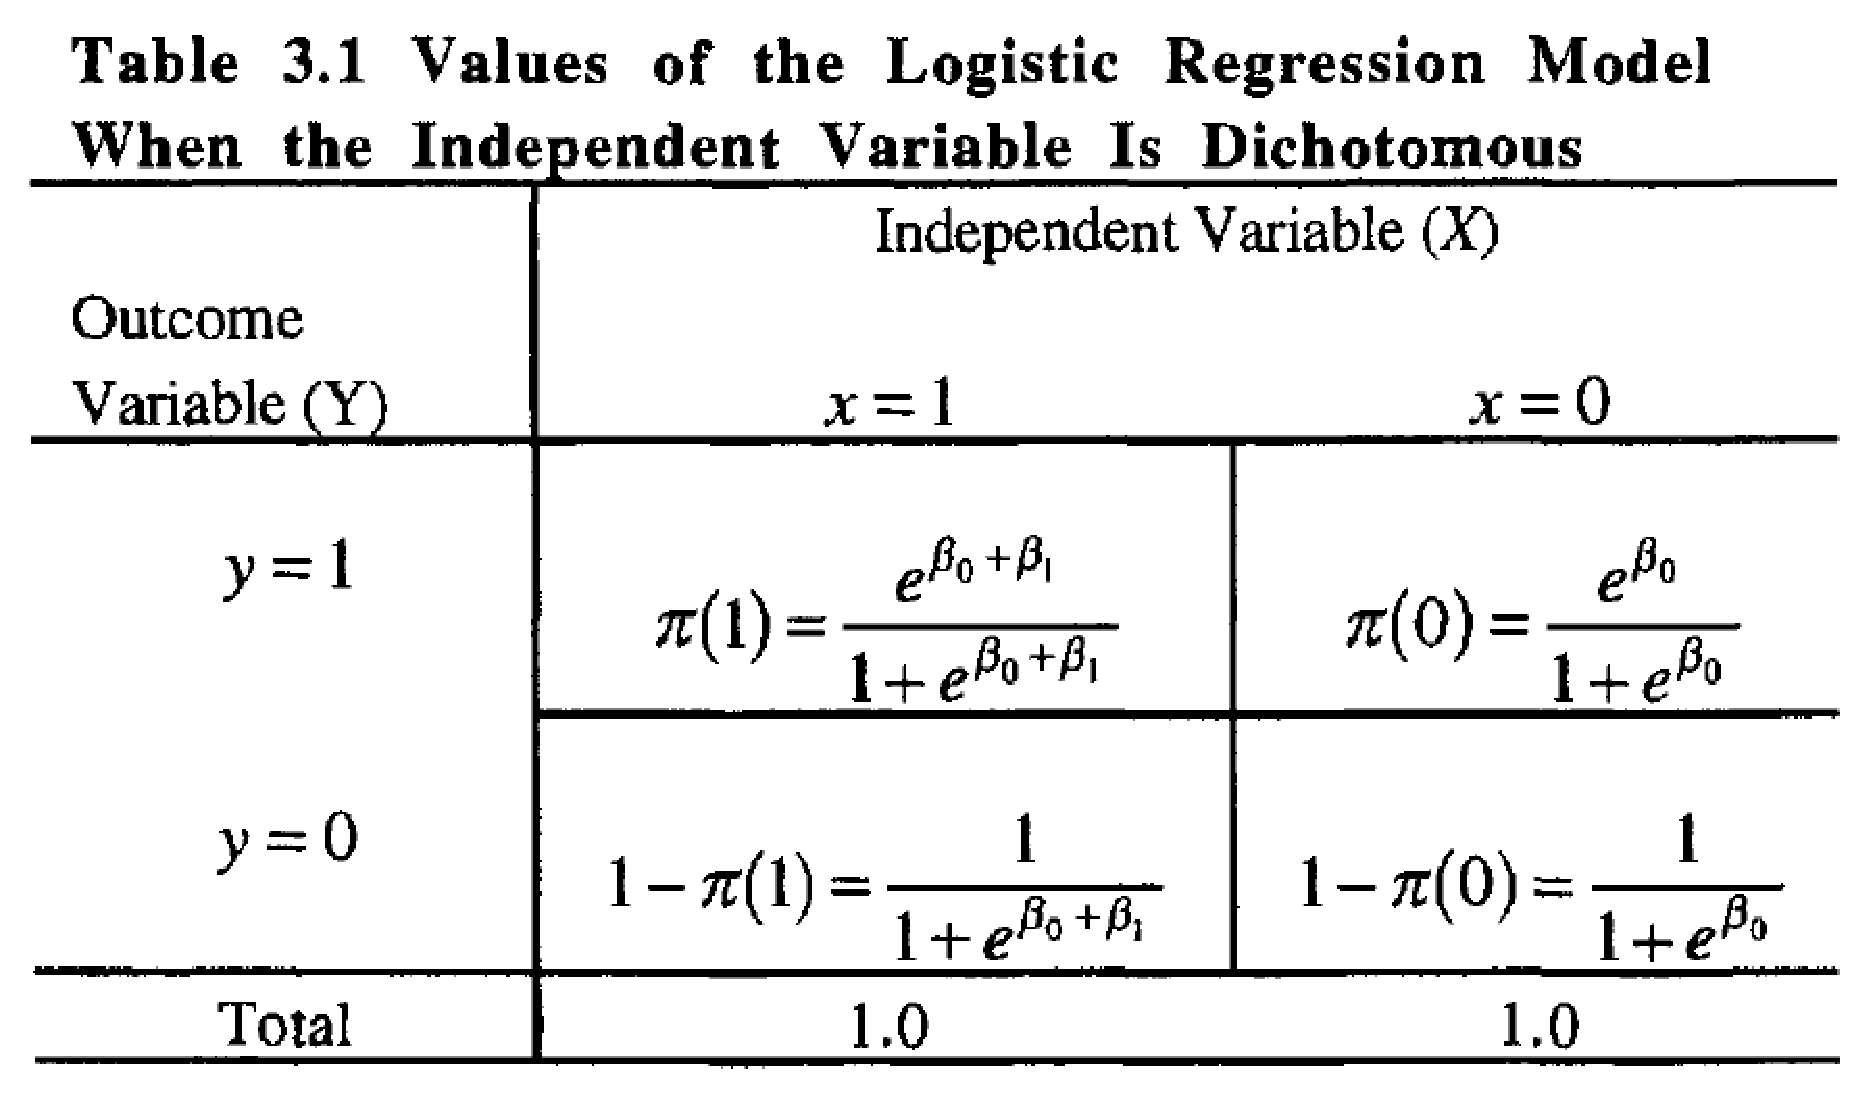
\includegraphics[scale = 0.35]{pictures/tbl_3_1.eps}
\caption{Hodnoty jednorozměrného logistického regresního modelu pro binární nezávislou veličinu}
\label{tbl_3_1}
\end{figure}

Důležitou statistikou používanou při analýze logistického regresního modelu je tzv. podíl rizik (odd ratio), které je definovaný jako
\begin{equation}
OR = \frac{\pi(1) / [1 - \pi(1)]}{\pi(0) / [1 - \pi(0)]}.
\end{equation}
V případě jednorozměrné logistické regrese s binární nezávislou veličinou, která nabývá hodnot 0 nebo 1, je vztah mezi podílem rizik a hodnotou regresního parametru definován jako
\begin{equation}
OR = \frac{\pi(1) / [1 - \pi(1)]}{\pi(0) / [1 - \pi(0)]} = \frac{\frac{e^{\beta_0 + \beta_1}}{1 + e^{\beta_0 + \beta_1}} \Big/ \frac{1}{1 + e^{\beta_0 + \beta_1}}}{\frac{e^{\beta_0}}{1 + e^{\beta_0}} \Big/ \frac{1}{1 + e^{\beta_0}}} = \frac{e^{\beta_0 + \beta_1}}{e^{\beta_0}} = e^{(\beta_0 + \beta_1) - \beta_0} = e^{\beta_1}.
\end{equation}
Podíl rizik přibližně vyjadřuje kolikrát je pravděpodobnější výskyt pozitivní hodnoty závislé veličiny pro pozorování $x = 1$ než pro pozorování $x = 0$. Pokud např. $y$ označuje výskyt / absenci rakoviny plic $x$ obsahuje informaci o tom, zda-li je daná osoba kuřák, pak $\widehat{OR} = 2$ znamená, že pravděpodobnost výskytu rakoviny plic u kuřáka je dvakrát vyšší než u nekuřáka. Vzhledem k definici podílu rizik je zřejmé, že tato statistika přibližně vyjadřuje tzv. relativní riziko, které je definováno jako $\pi(1) / \pi(0)$. Z tabulky (3.1) je pak zřejmé, že tato aproximace platí, pokud $[1 - \pi(0)] / [1 - \pi(1)] \approx 1$. To je splněno, pokud $\pi(x)$ je malé jak pro $x = 1$ tak pro $x = 0$.

V řadě aplikací logistické regrese, se kterými se můžeme setkat v odborné literatuře, jsou spojité numerické veličiny převedeny na binární pomocí vhodně zvoleného hraničního bodu. Pro ilustraci uvádíme klasifikační tabulku (3.2), kdy veličina $AGED$ nabývá hodnoty 0 pokud je dané osobě méně než 55 let a hodnoty 1 v ostatních případech.
\begin{figure}[htp]
\centering
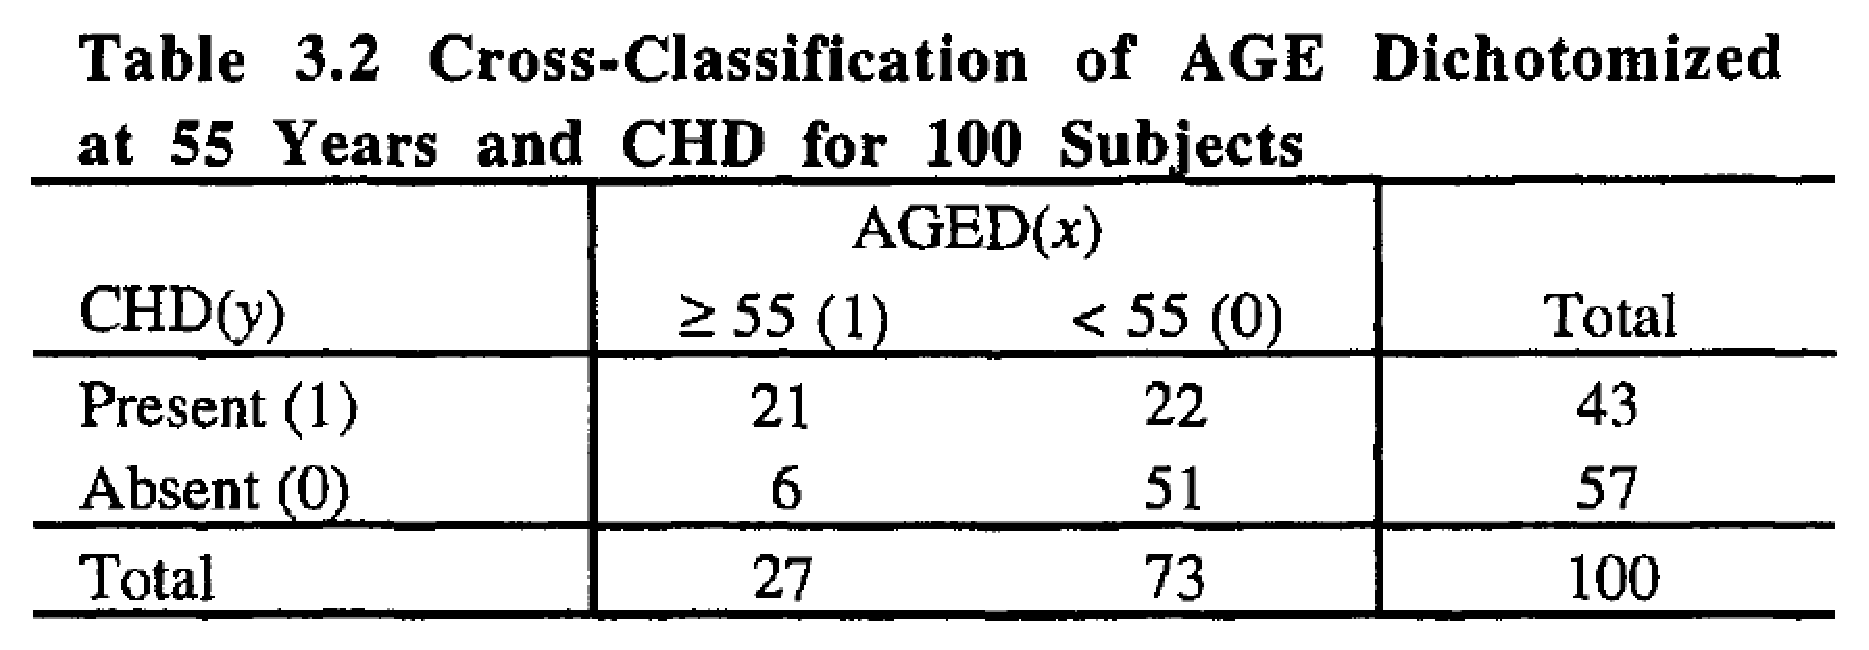
\includegraphics[scale = 0.35]{pictures/tbl_3_2.eps}
\caption{Klasifikační tabulka pro binární nezávislou veličinu $AGED$ a závislou veličinu $CHD$ představující výskyt ischemické choroby srdeční.}
\label{tbl_3_2}
\end{figure}
Zkoumaná populace se dle tabulky (3.2) skládala z 21 osob s hodnotami $(x = 1, y = 1)$, 22 osob s hodnotami $(x = 0, y = 1)$, 6 osob s hodnotami $(x = 1, y = 0)$ a 51 osob s hodnotami $x = 0, y = 0$. Pokud bychom na základě těchto dat odhadli metodou maximální věrohodnosti parametr pro veličinu $AGED$, získali bychom hodnotu 2.094. Podíl rizik bychom pak odhadli na $\widehat{OR} = e^{2.094} = 8.1$. Podíl rizik však lze odhadnout také přímo s pomocí klasifikační tabulky, tj. jako
\begin{equation}
\widehat{OR} = \frac{\hat{\pi}(1) / [1 - \hat{\pi}(1)]}{\hat{\pi}(0) / [1 - \hat{\pi}(0)]} = \frac{21/6}{22/51} = 8.11.
\end{equation}
Interval spolehlivosti podílu rizik se pak určí tak, že se nejprve vypočtou krajní hodnoty odpovídající intervalu spolehlivosti odhadu parametru $\beta_1$ a na ně se aplikuje exponenciála, tj.
\begin{equation}
e^{\beta_1 \pm z_{1 - \alpha / 2} \widehat{se}(\hat{\beta}_1)}.
\end{equation}
Vzhledem ke způsobu konstrukce je interval spolehlivosti podílu rizik nesymetrický.

V předchozím textu jsme předpokládali, že nezávislá binární veličina $x$ nabývá veličin 0 a 1. Je třeba zdůraznit, že výše uvedené závěry jsou platné pouze pro tento případě. Uvažujme situaci, kdy $x$ nabývá dvou různých obecných hodnot $a$ a $b$. Pak platí
\begin{equation}
\ln[\widehat{OR}(a, b)] = \hat{g}(x = a) - \hat{g}(x = b) = (\hat{\beta}_0 + \hat{\beta}_1 a) - (\hat{\beta}_0 + \hat{\beta}_1 b) = \hat{\beta}_1 (a - b)
\end{equation}
neboli
\begin{equation}
\widehat{a, b} = e^{\hat{\beta}_1 (a - b)}.
\end{equation}
Analogie (3.2) pak má podobu
\begin{equation}
\widehat{OR}(a, b) = \frac{\hat{\pi}(x = a) / [1 - \hat{\pi}(x = a)]}{\hat{\pi}(x = b) / [1 - \hat{\pi}(x = b)]}.
\end{equation}
Interval spolehlivosti podílu rizik lze vyjádřit jako
\begin{equation}
e^{\hat{\beta}_1(a - b) \pm z_{1 - \alpha / 2}|a - b| \widehat{se}(\hat{\beta}_1)}.
\end{equation}
Je třeba zdůraznit, že kódování binární proměnné do 0 a 1 je zdaleka nejčastější, a proto ho budeme používat i v následujícím textu. Dalším používaným kódováním je pak -1 a 1, které je však méně frekventované.

\section{Nezávislá kategorická veličina}

Kategorickou veličinou rozumíme veličinu, která může nabývat $k > 2$ různých nominální hodnot. Jak jsme již zmínili výše, takovouto veličinu musíme převést na $k - 1$ pomocných binárních veličin. Jako příklad uveďme veličinu $X_i$, která nabývá hodnot 0 pro bělocha, 1 pro černocha a 2 pro asiata. Tuto veličinu musíme nahradit dvojicí pomocných binárních veličin $D_{i1}$ a $D_{i2}$. Při nejčastěji používaném kódování nabývá veličina $D_{i1}$ hodnoty 1, pokud je daná osoba černoch, a 0 v ostatních případech. Podobně veličina $D_{i2}$ nabývá hodnoty 1, pokud je daná osoba asiat, a 0 v ostatních případech. Je třeba zdůraznit, že pokud bych do modelu přidali ještě třetí veličinu, $D_{i3}$, která by nabývala hodnoty 1, pokud je daná osoba běloch, a 0 v ostatních případech, vytvořili bychom perfektní multikolinearitu.\footnote{Informaci o tom, že je daná osoba běloch totiž, lze získat také na základě veličin $D_{i1}$ a $D_{i2}$. Konkrétně, pokud obě veličiny nabývají hodnoty 0, víme, že se nejedná ani o černocha a ani o asiata, takže se musí jednat o bělocha. Informace představovaná veličinou $D_{i3}$ je tak duplicitní.}

Pro ilustraci uvažujme model $y(\pmb{x}) = \beta_0 + \beta_1 D_{i1} + \beta_2 D_{i2}$, kde $y = 1$ představuje výskyt ischemické choroby srdeční. Pokud použijeme standardní kódování pomocných binárních veličin na hodnoty 0 a 1, platí
\begin{equation}
\ln[\widehat{OR}(\textit{black}, \textit{white})] = \hat{g}(\textit{black}) - \hat{g}(\textit{white}) = (\hat{\beta}_0 + \hat{\beta}_1 \cdot 1 + \hat{\beta}_2 \cdot 0) - (\hat{\beta}_0 + \hat{\beta}_1 \cdot 0 + \hat{\beta}_2 \cdot 0) = \hat{\beta}_1.
\end{equation}
Jak vyplývá z označení $\widehat{OR}(\textit{black}, \textit{white})$, vyjadřuje $\hat{\beta}_1$ odhad, kolikrát je výskyt ischemické choroby srdeční pravděpodobnější u černocha než u bělocha.  Pokud bychom chtěli porovnat pravděpodobnosti výskytu ischemické choroby srdeční pro černocha vs. asiata, museli bychom výše uvedenou rovnici upravit do tvaru
\begin{multline}
\ln[\widehat{OR}(\textit{black}, \textit{asian})] = \hat{g}(\textit{black}) - \hat{g}(\textit{asian}) =\\(\hat{\beta}_0 + \hat{\beta}_1 \cdot 1 + \hat{\beta}_2 \cdot 0) - (\hat{\beta}_0 + \hat{\beta}_1 \cdot 0 + \hat{\beta}_2 \cdot 1) = \hat{\beta}_1 - \hat{\beta}_2.
\end{multline}
Interval spolehlivosti $\widehat{OR}(\textit{black}, \textit{white})$ pak má podobu
\begin{equation}
e^{\hat{\beta}_1 \pm z_{1 - \alpha / 2} \sqrt{\widehat{var}\big(\ln[\widehat{OR}(\textit{black}, \textit{white})]\big)}} = e^{\hat{\beta}_1 \pm z_{1 - \alpha / 2} \widehat{se}(\hat{\beta}_1)}
\end{equation}
a interval spolehlivosti $\widehat{OR}(\textit{black}, \textit{asian})$ podobu
\begin{equation}
e^{(\hat{\beta}_1 - \hat{\beta}_2) \pm z_{1 - \alpha / 2} \sqrt{\widehat{var}\big(\ln[\widehat{OR}(\textit{black}, \textit{asian})]\big)}},
\end{equation}
kde
\begin{equation}
\widehat{var}\big(\ln[\widehat{OR}(\textit{black}, \textit{asian})]\big) = \widehat{var}(\hat{\beta}_1) - 2 \hat{\beta}_1 \hat{\beta}_2 \widehat{cov}(\hat{\beta}_1, \hat{\beta}_2) + \widehat{var}(\hat{\beta}_2).
\end{equation}

Dalším možným způsobem kódování je použití hodnot -1, 0 a 1. Běloch je tak reprezentován hodnotami -1 pro $D_{i1}$ a -1 pro $D_i2$, černoch hodnotami 1 pro $D_{i1}$ a 0 pro $D_{i2}$ a konečně asiat hodnotami 0 pro $D_{i1}$ a 1 pro $D_{i2}$. Platí tedy
\begin{equation}
\ln[\widehat{OR}(\textit{black}, \textit{white})] = \hat{g}(\textit{black}) - \hat{g}(\textit{white}) = (\hat{\beta}_0 + \hat{\beta}_1 \cdot 1 + \hat{\beta}_2 \cdot 0) - (\hat{\beta}_0 + \hat{\beta}_1 \cdot (-1) + \hat{\beta}_2 \cdot (-1)) = 2\hat{\beta}_1 + \hat{\beta}_2
\end{equation}
a podobně
\begin{equation}
\ln[\widehat{OR}(\textit{black}, \textit{asian})] = \hat{g}(\textit{black}) - \hat{g}(\textit{asian}) = (\hat{\beta}_0 + \hat{\beta}_1 \cdot 1 + \hat{\beta}_2 \cdot 0) - (\hat{\beta}_0 + \hat{\beta}_1 \cdot 0 + \hat{\beta}_2 \cdot 1) = \hat{\beta}_1 - \hat{\beta}_2
\end{equation}.
Intervaly spolehlivosti podílů rizik pak mají podobu
\begin{equation}
e^{(2\hat{\beta}_1 + \hat{\beta}_2) \pm z_{1 - \alpha / 2} \sqrt{\widehat{var}\big(\ln[\widehat{OR}(\textit{black}, \textit{white})]\big)}}
\end{equation}
pro $\widehat{OR}(\textit{black}, \textit{white})$ a
\begin{equation}
e^{(\hat{\beta}_1 - \hat{\beta}_2) \pm z_{1 - \alpha / 2} \sqrt{\widehat{var}\big(\ln[\widehat{OR}(\textit{black}, \textit{asian})]\big)}}
\end{equation}
pro $\widehat{OR}(\textit{black}, \textit{asian})$ kde
\begin{equation}
\widehat{var}\big(\ln[\widehat{OR}(\textit{black}, \textit{white})]\big) = 4\widehat{var}(\hat{\beta}_1) + 4 \hat{\beta}_1 \hat{\beta}_2 \widehat{cov}(\hat{\beta}_1, \hat{\beta}_2) + \widehat{var}(\hat{\beta}_2).
\end{equation}
a
\begin{equation}
\widehat{var}\big(\ln[\widehat{OR}(\textit{black}, \textit{asian})]\big) = \widehat{var}(\hat{\beta}_1) - 2 \hat{\beta}_1 \hat{\beta}_2 \widehat{cov}(\hat{\beta}_1, \hat{\beta}_2) + \widehat{var}(\hat{\beta}_2).
\end{equation}
Tento způsob kódování je však používán spíše výjimečně, a proto budeme v následujícím textu používat kódování pomocí hodnot 0 a 1.

\end{document}
